\section{实验流程}

\begin{figure}[H]
  \centering
  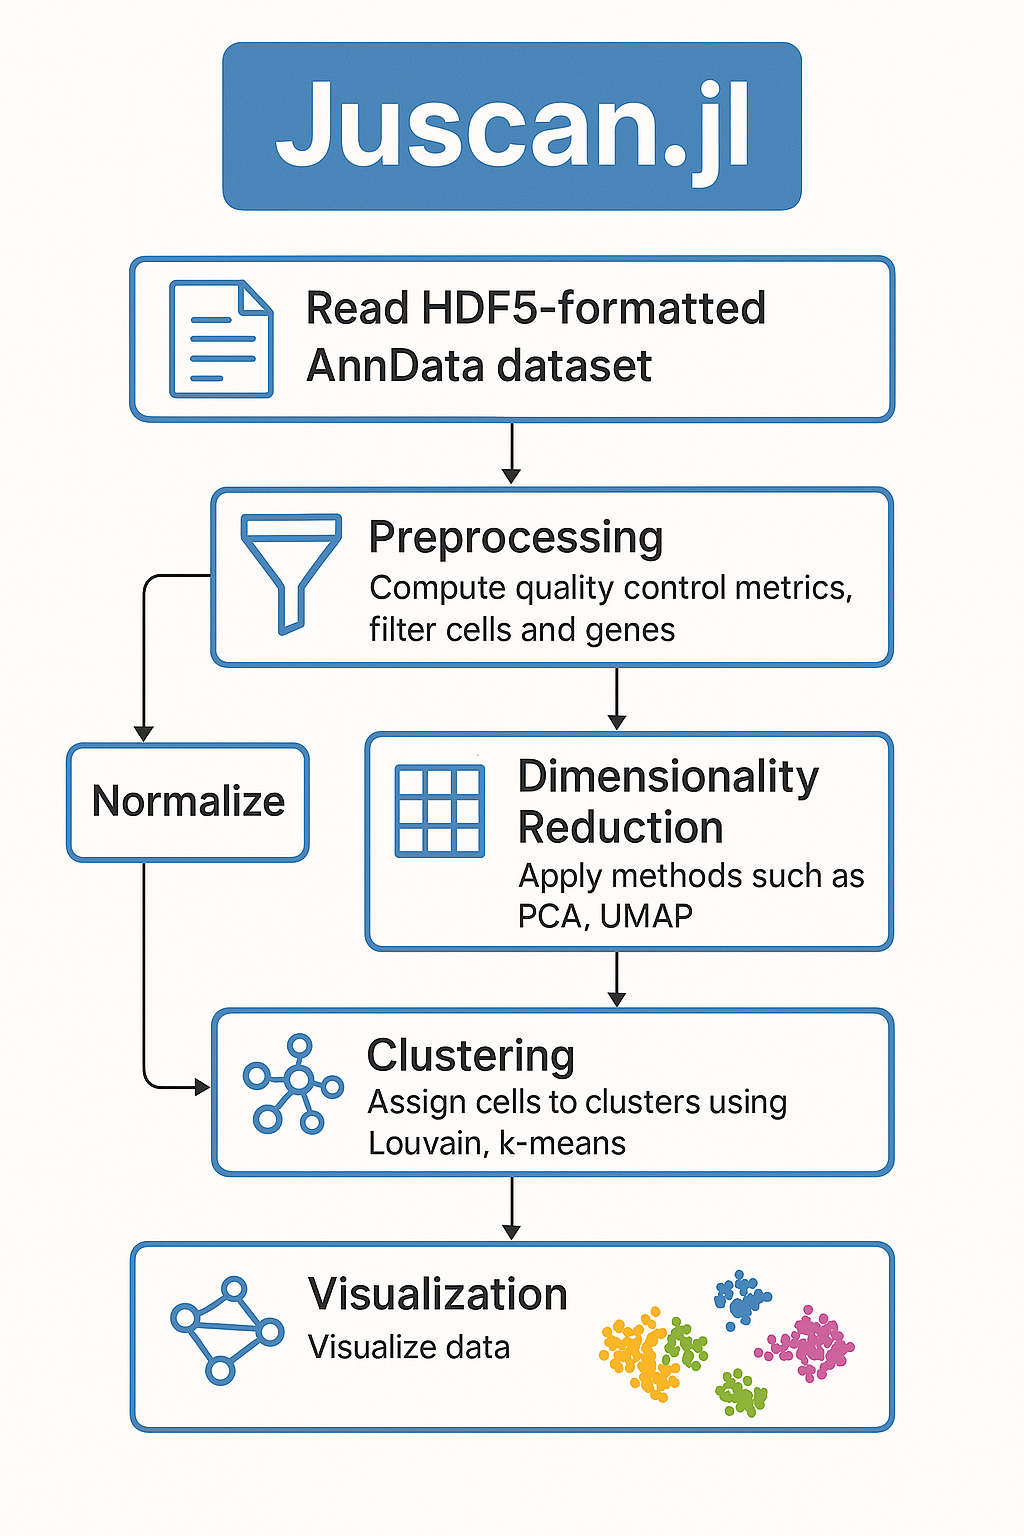
\includegraphics[width=0.57\textwidth]{img/flow_chart.png}
  \caption{实验流程}
  \label{fig:flow_chart}
\end{figure}

\section{实验方法}

\subsection{扩增插入基因}

\textbf{一、引物设计}

\begin{enumerate}[itemsep=0.1em]
\item 使用高质量的模板。
\item 勿使用dUTP和带有尿嘧啶的引物和模板。
\item 如实验需要,可适当提高Phanta酶的使用量,但50ul体系内酶量建议不要超过2ul。
\item Phanta酶具有较强的校对活性。因此,如扩增产物需要进行TA克隆,加之前必须进行DNA纯化。
\item 为了防止Phanta酶的校对活性降解引物,在配制反应体系时请最后加入聚合酶。
\item 引物设计
\begin{enumerate}[label={(\arabic*)}, itemsep=0.1em]
  \item 引物3端最后一个碱基最好为G或者C;
  \item 引物3端最后8个碱基应避免出现连续错配;
  \item 引物3端应避免出现发夹结构;
  \item 正向引物和反向引物的Tm值相差不超过1℃为佳,Tm值调整至55~65℃为佳;
  \item 引物额外附加序列,即与模板非配对序列,不应参与引物Tm值计算
  \item 引物的GC含量控制在40\%-60\%之间;
  \item 引物A、G、C、T整体分布要尽量均匀,避免使用GC或者AT含量高的区域;
  \item 引物内部或者两条引物之间避免有5个碱基以上的互补序列,两条引物的3端避免有3个碱基以上的互补序列;
  \item 引物设计完毕请使用NCBI BLAST功能检索引物特异性,以避免非特异性扩增产生。
\end{enumerate}
\end{enumerate}

\textbf{二、PCR}(Panta酶反应体系,从全基因组中PCR结束之后需要做一步消化。要注意全程在冰上操作,加的体积从大到小)

\begin{longtable}{cc}
  \caption{PCR 反应体系} \\
  \toprule
  \textbf{组分} & \textbf{体积} \\
  \midrule

  ddH$_2$O & 17~$\mu$l(加到 50~$\mu$l) \\
  2$\times$Buffer & 25~$\mu$l \\
  dNTP & 1~$\mu$l \\
  上、下游引物(分开加) & 2~$\mu$l \\
  酶 & 1~$\mu$l \\
  模板 DNA & 2~$\mu$l \\

  \bottomrule
\end{longtable}


\begin{longtable}{ccc}
  \caption{PCR 反应条件} \\
  \toprule
  \textbf{步骤} & \textbf{时间} & \textbf{温度} \\
  \midrule
  \endfirsthead

  \multicolumn{3}{l}{\textit{续表:PCR 反应条件}} \\
  \toprule
  \textbf{步骤} & \textbf{时间} & \textbf{温度} \\
  \midrule
  \endhead

  \bottomrule
  \multicolumn{3}{r}{\textit{表格接下页}} \\
  \endfoot

  \bottomrule
  \endlastfoot

  预变性 & 3 min & 95$^\circ$C \\
  变性   & 15 sec & 95$^\circ$C \\
  退火   & 15 sec & 60$^\circ$C(根据引物 Tm 值调整) \\
  延伸   & 150 sec(根据 bp 长度调整) & 72$^\circ$C \\
  彻底延伸 & 5 min & 72$^\circ$C \\

\end{longtable}

\textbf{三.跑胶}

\begin{enumerate}[itemsep=0.1em]
  \item 安仪器,根据要跑胶的基因数目的具体情况计算要用到的梳子种类和皿的种类。
  \item 加溶剂,两次煮沸,在侧面冷水下冲洗到$50^\circ\text{C}$。
  \item 加核酸染料。
  \item 倒胶。
  \item 晾干30min,待胶条凝固冷却成型。
  \item 取梳子。
  \item 转胶条。
  \item 加基因和marker。
  \item 电压150V,电流400A,跑胶。
\end{enumerate}

\textbf{四.胶回收}

\begin{enumerate}[itemsep=0.1em]
  \item 切胶,置于2.0ml EP管中。切胶要放切胶板,切完的胶扔到红色垃圾袋,管中的胶放在相应的引物旁边,作好引物名称标记。
  \item 加3倍凝胶体积的Buffer MB,$55^\circ\text{C}$水浴加热,直至凝胶全部融化。
  \item 在等待胶溶期间,向离心吸附柱中加入500$\mu$l Buffer BL,静止1min,室温下12,000rpm离心1min,弃收集管中的废液,将离心吸附柱重新放回收集管中。
  \item 待凝胶溶液冷却至室温后,转移到离心吸附柱内,静置1min,室温下12,000rpm离心1min。
  \item 弃除收集管中的废液,将离心吸附柱重新插回收集管中。
  \item 加入600$\mu$l Buffer MW于离心吸附柱中,室温下12,000rpm离心30s,弃除收集管中的废液,将离心吸附柱重新插回收集管中。
  \item 重复操作步骤6。
  \item 室温下12,000rpm空离2min,弃除收集管。
  \item 将吸附柱置于1.5ml离心管中,加入50$\mu$l\~100$\mu$l至吸附柱中央,室温静置1min,12,000rpm离心1min。
  \item 弃去吸附柱,获得的DNA片段可直接用于后续反应或于$-20^\circ\text{C}$长期保存。
\end{enumerate}

\subsection{扩增质粒}

\textbf{一.摇菌(扩增质粒数量)}

\textbf{二.提质粒}

\begin{enumerate}[itemsep=0.3em]
  \item 取摇菌管,4000rpm离心3min。弃去培养基,将摇菌管倒扣于吸水纸上吸尽残液。
  \item 向留有菌体沉淀的摇菌管中加入250$\mu$l Buffer P1,用移液器或涡旋振荡混匀后将其转入1.5ml离心管中。
  \item 向步骤2中加入250$\mu$l Buffer P2,温和地上下颠倒混匀8–10次,使菌体充分裂解。
  \item 向步骤3中加入350$\mu$l Buffer P3,立即温和地上下颠倒8–10次使溶液彻底中和。将混合液加入吸附柱中,12,000rpm离心30–60s,弃废液并将吸附柱重新放回收集管中。
  \item 重复步骤4。
  \item 将吸附柱放入新的1.5ml离心管中,12,000rpm离心2min,以干燥吸附柱,彻底去除残留漂洗液。
  \item 将吸附柱再次置于新的灭菌1.5ml离心管中,加入30$\mu$l无菌水至吸附柱膜中央,室温静置2min,12,000rpm离心1min以洗脱DNA。
  \item 测定质粒DNA浓度,并在离心管上做好标记。
\end{enumerate}

\subsection{构建新的质粒}

\textbf{一、酶切}

\begin{longtable}{cc}
  \caption{酶切体系} \\
  \toprule
  \textbf{组分} & \textbf{用量} \\
  \midrule
  \endfirsthead

  \multicolumn{2}{l}{\textit{续表:酶切体系}} \\
  \toprule
  \textbf{组分} & \textbf{用量} \\
  \midrule
  \endhead

  \bottomrule
  \endfoot

  \bottomrule
  \endlastfoot

  Plasmid & 2~$\mu$g \\
  Enzyme 1 & 1~$\mu$l \\
  Enzyme 2 & 1~$\mu$l \\
  10$\times$酶切 Buffer & 3~$\mu$l \\
  ddH$_2$O & up to 30~$\mu$l \\
  
\end{longtable}

震荡混匀,37$^\circ\text{C}$酶切30min(3000bp酶切30min)

\textbf{二、纯化}(与胶回收的原理和步骤类似)

\textbf{三、连接}

弹管混匀后冰浴30min

\begin{longtable}{cc}
  \caption{连接体系} \\
  \toprule
  \textbf{组分} & \textbf{用量} \\
  \midrule
  \endfirsthead

  \multicolumn{2}{l}{\textit{续表:连接体系}} \\
  \toprule
  \textbf{组分} & \textbf{用量} \\
  \midrule
  \endhead

  \bottomrule
  \endfoot

  \bottomrule
  \endlastfoot

  载体 & 30~ng(3~$\mu$l / 2~$\mu$l) \\
  插入序列 & 50~ng(5~$\mu$l / 6~$\mu$l) \\
  10$\times$酶切 Buffer & 1~$\mu$l \\
  Exo3 & 1~$\mu$l(取 1~$\mu$l 加到 9~$\mu$l 水中,稀释 10 倍后取 1~$\mu$l) \\
\end{longtable}

\textbf{四.转化}

\begin{enumerate}[itemsep=0.1em]
  \item 取感受态细胞放冰上解冻。
  \item 向感受态细胞中加入10$\mu$l连接产物,弹管混匀。
  \item 冰浴10min。
  \item 42$^\circ$\text{C}热激90s。
  \item 冰浴3\~5min。
  \item 在超净台中加入1ml不含抗生素的LB培养基,混匀后于37$^\circ$\text{C}孵育1h。
  \item 5,000rpm离心4min,吸走上清,只留100$\mu$l,吹打重悬后涂布于抗性平板上。
  \item 置于37$^\circ$\text{C}培养10–16h。
  \item 挑取单克隆接种至含抗生素的LA液体培养基中,小摇培养约3h。
\end{enumerate}

\textbf{注意:}需要设置一个阴性对照——酶切后的载体(3$\mu$l,无需添加连接酶),用于判断载体是否被完全切开或发生自我连接。

\subsection{PCR 验证和测序}

\textbf{一、菌液PCR}

\textbf{二、跑胶验证}

\subsection{RNAi 实验}

\begin{enumerate}[itemsep=0.3em]

  \item 第0天:在含抗生素的LB液体培养基中接种含有RNAi质粒的HT115大肠杆菌,于37$^\circ$\text{C}震荡培养12–16小时,以获取最多的活菌。
  
  \item 第一天:
  \begin{enumerate}[label*={(\alph*)}, itemsep=0.3em]
    \item 将菌液1:100稀释至2$\times YT ^+$ 抗生素中,培养至OD$_{595}$ = 0.4;
    \item 加入无菌 IPTG 使终浓度达到0.4mM,在37$^\circ$\text{C}摇床诱导4小时;
    \item 在含抗生素和IPTG的培养条件下继续培养。可直接使用培养液,也可将菌液以2000rpm离心、吸走上清后重悬浓缩细胞,然后播种至RNAi平板上。
  \end{enumerate}
  
  \item 挑选线虫至RNAi平板上,开始RNAi实验。
  
\end{enumerate}

\subsection{Smurf Assy 实验}

\begin{enumerate}[itemsep=0.1em]
  \item 提前一天使用LB培养基摇菌OP50(线虫的食物),于37$^\circ$\text{C}培养12–16小时。使用前将菌液浓缩10倍。
  \item 配制5\% Smurf染液:在浓缩后的菌液中加入0.25g Smurf染料粉末,加入5ml浓缩菌液,涡旋混匀备用。
  \item 用2ml离心管,加入200$\mu$l M9缓冲液,将待处理线虫挑入管中。再加入400$\mu$l步骤2中配制的5\% Smurf染液。
  \item 将混合液放置在20$^\circ$\text{C}水平摇床上,缓慢摇晃3小时。
  \item 使用台式小型离心机离心10s,使线虫沉降至管底。吸去上清,保留约300$\mu$l液体,补加1ml M9,轻轻重悬清洗。重复洗涤多次,直到线虫体表的蓝色染料明显变淡,能透过离心管看到手指为止。最后保留约300$\mu$l液体。
  \item 将洗后的线虫液体,用低吸附枪头滴加在已吹干的NGM平板上,轻轻摇晃,使液体尽可能摊平于平板表面。从该平板中挑取线虫转移到无菌NGM平板(用于拍照)。
  \item 在无菌NGM平板上加入叠氮化钠杀死线虫,排列整齐后进行拍照观察。根据Smurf染料在虫体内的渗透程度,判断线虫肠道屏障的完整性。
\end{enumerate}

\subsection{荧光共聚焦实验}


\begin{enumerate}[itemsep=0.1em]
\item 使用左旋咪唑麻醉线虫,将线虫进行排列(每个RNAi组拍摄大约30条虫子)。
\item 使用488nm波长的荧光通道,拍摄线虫表皮细胞间HMR-1-GFP的点状荧光信号。
\end{enumerate}

\section{小结}

本章节详细描述了从基因扩增到荧光共聚焦实验的完整实验步骤,涵盖了DNA操作,RNAi实验以及线虫屏障相关实验多个环节。整个实验流程设计严谨,步骤清晰,我们的实验确保了每一步操作的准确性和可重复性,为研究基因功能和线虫生物学特性提供了可靠的实验方法。

我们的实验首先从引物设计开始,整个引物设计规则严谨,为了确保后续的一系列实验按部就班开展。在扩增插入基因时,我们使用Phanta酶进行PCR反应, PCR产物会通过跑胶和胶回收进行纯化。接下来是质粒的扩增和提取。我们通过摇菌培养细菌以扩增质粒数量,然后进行质粒提取,最终获得高纯度质粒DNA。在构建新的质粒时,我们首先对质粒进行酶切,酶切后的载体通过纯化去除杂质,然后与插入目的片段进行连接,连接产物又通过转化进入感受态细胞,经过培养后在氨苄板上筛选阳性克隆。为了验证阳性克隆,本实验采用菌液PCR和跑胶验证,以确保插入序列的正确性。

随后我们进行RNAi实验。首先我们在LB培养基中培养HT115菌株,加入IPTG诱导dsRNA表达涂板。然后我们将线虫转移到RNAi平板上进行喂养。Smurf Assay实验用于评估线虫肠道屏障功能,利用浓缩菌液配制5\%的 Smurf染料,对线虫进行染色后通过离心、洗涤和显微镜观察得出线虫肠道屏障损伤程度结果。最后,荧光共聚焦拍摄和判断线虫表皮屏障的受损情况。最后两种判断线虫屏障受损与否的实验结果我们都将用定量软件进行分析,以确保最终的实验结论严谨可靠。
